\documentclass[preprint, 3p,
authoryear]{elsarticle} %review=doublespace preprint=single 5p=2 column
%%% Begin My package additions %%%%%%%%%%%%%%%%%%%

\usepackage[hyphens]{url}

  \journal{An awesome journal} % Sets Journal name

\usepackage{lineno} % add

\usepackage{graphicx}
%%%%%%%%%%%%%%%% end my additions to header

\usepackage[T1]{fontenc}
\usepackage{lmodern}
\usepackage{amssymb,amsmath}
\usepackage{ifxetex,ifluatex}
\usepackage{fixltx2e} % provides \textsubscript
% use upquote if available, for straight quotes in verbatim environments
\IfFileExists{upquote.sty}{\usepackage{upquote}}{}
\ifnum 0\ifxetex 1\fi\ifluatex 1\fi=0 % if pdftex
  \usepackage[utf8]{inputenc}
\else % if luatex or xelatex
  \usepackage{fontspec}
  \ifxetex
    \usepackage{xltxtra,xunicode}
  \fi
  \defaultfontfeatures{Mapping=tex-text,Scale=MatchLowercase}
  \newcommand{\euro}{€}
\fi
% use microtype if available
\IfFileExists{microtype.sty}{\usepackage{microtype}}{}
\usepackage[]{natbib}
\bibliographystyle{plainnat}

\ifxetex
  \usepackage[setpagesize=false, % page size defined by xetex
              unicode=false, % unicode breaks when used with xetex
              xetex]{hyperref}
\else
  \usepackage[unicode=true]{hyperref}
\fi
\hypersetup{breaklinks=true,
            bookmarks=true,
            pdfauthor={},
            pdftitle={Title of the paper},
            colorlinks=true,
            urlcolor=blue,
            linkcolor=blue,
            pdfborder={0 0 0}}

\setcounter{secnumdepth}{5}
% Pandoc toggle for numbering sections (defaults to be off)


% tightlist command for lists without linebreak
\providecommand{\tightlist}{%
  \setlength{\itemsep}{0pt}\setlength{\parskip}{0pt}}






\begin{document}


\begin{frontmatter}

  \title{Title of the paper}
    \author[ENSGSI]{Alice Anonymous%
  \corref{cor1}%
  \fnref{1}}
   \ead{alice@example.com} 
      \affiliation[ENSGSI]{Universite de Lorraine, ENSGSI, 8 Rue
Bastien-Lepage, 54000 Nancy, France}
    \cortext[cor1]{Corresponding author}
    \fntext[1]{This is the first author footnote.}
    \fntext[2]{Another author footnote.}
  
  \begin{abstract}
  This is the abstract of Max 300 Words.

  \href{https://doi.org/10.1007/978-981-16-5248-6_15}{Take as
  inspiration}
  \end{abstract}
    \begin{keyword}
    keyword1 \sep keyword2 \sep 
    keyword2
  \end{keyword}
  
 \end{frontmatter}

\hypertarget{introduction-max-1.5-pages}{%
\section{Introduction {[}Max 1.5
pages{]}}\label{introduction-max-1.5-pages}}

\begin{itemize}
\tightlist
\item
  Present the context.
\item
  Presentation of the problematic.

  \begin{itemize}
  \tightlist
  \item
    Explain why is it important and relevant.
  \item
    For whom is important the problem?
  \end{itemize}
\item
  Clearly the research question that the paper wants to answer
\end{itemize}

\hypertarget{methodology-of-literature-review-max-1-pag.}{%
\section{Methodology of literature review {[}Max 1
pag.{]}}\label{methodology-of-literature-review-max-1-pag.}}

\begin{itemize}
\tightlist
\item
  Present the literature protocol

  \begin{itemize}
  \tightlist
  \item
    Selection of the Keywords, search equations, databases
  \end{itemize}
\item
  Grid lecture of the articles.
\end{itemize}

\hypertarget{results-max-3-pages}{%
\section{Results {[}Max 3 pages{]}}\label{results-max-3-pages}}

\begin{itemize}
\tightlist
\item
  Table the articles
\item
  Quantitative analysis
\item
  Qualitative analysis
\end{itemize}

\hypertarget{equations}{%
\subsection{Equations}\label{equations}}

Here is an equation: \[ 
  f_{X}(x) = \left(\frac{\alpha}{\beta}\right)
  \left(\frac{x}{\beta}\right)^{\alpha-1}
  e^{-\left(\frac{x}{\beta}\right)^{\alpha}}; 
  \alpha,\beta,x > 0 .
\]

Here is another: \begin{align}
  a^2+b^2=c^2.
\end{align}

Inline equations: \(\sum_{i = 2}^\infty\{\alpha_i^\beta\}\)

\hypertarget{figures-and-tables}{%
\subsection{Figures and tables}\label{figures-and-tables}}

Figure \ref{fig2} is generated using an R chunk.

\begin{figure}

{\centering 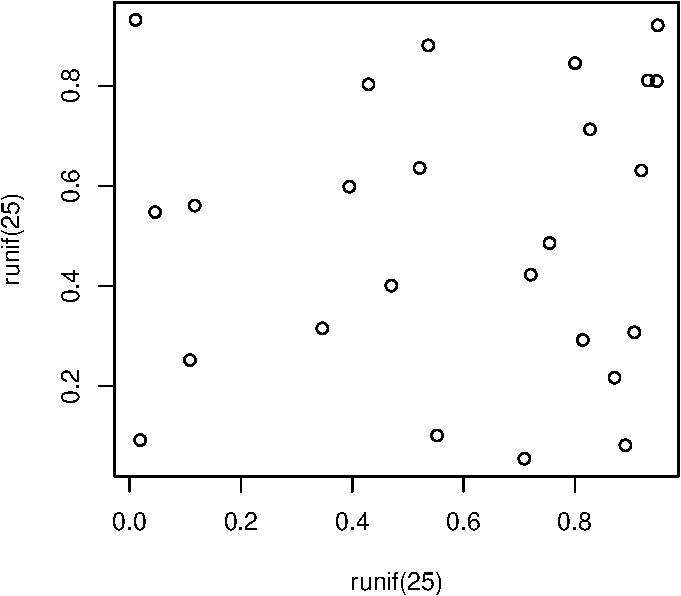
\includegraphics[width=0.5\linewidth]{Article-template_files/figure-latex/fig2-1} 

}

\caption{\label{fig2}A meaningless scatterplot.}\label{fig:fig2}
\end{figure}

\hypertarget{discussion-2-3-pages}{%
\section{Discussion {[}2-3 pages{]}}\label{discussion-2-3-pages}}

\begin{itemize}
\item
  Analysis of the elements founded
\item
  Clearly define the limits of your approach.
\end{itemize}

\hypertarget{conclusion-1-page}{%
\section{Conclusion {[}1 page{]}}\label{conclusion-1-page}}

\begin{itemize}
\tightlist
\item
  Do we answer the research questions?
\item
  What do we learn and what need to be further explore
\end{itemize}

\renewcommand\refname{References}
\bibliography{mybibfile.bib}


\end{document}
